\documentclass[Bachelorarbeit.tex]{subfiles}
\begin{document}

\chapter{Appendix}
If not otherwise noted pictures are taken from \textit{Wikicommons}. http://commons.wikimedia.org
\addtocontents{toc}{\protect\setcounter{tocdepth}{1}}
%\ifthenelse{\equal{\getLanguage}{english}} % %prints just the list of acronyms
%  		{\addcontentsline{toc}{chapter}{Appendix}}
%  		{\addcontentsline{toc}{chapter}{Anhang}} 
\section{YCbCr-Color-Space}  	
\subsection{Color Spaces}
A color space is a mathematical model to represent color information out of a picture. There were several color models available:
\begin{itemize}
\item RGB based color space (RGB, normalized RGB)
\item Hue based color space (HSI, HSV and HSL)
\item Luminance based color space (YCbCr, YIQ and YUV)
\item Perceptually uniform color space (CIEXYZ, CIELAB, and CIELUV)
\end{itemize}

Luminance based color space has the split the image into intensity (luminance) informations and color (chrominance) informations. The YCbCr space was chosen because several articles recommended this color space for video applications (because of its speed).
\medskip
The letters of YCbCr represents:
\begin{itemize}
\item Y: luminance
\item Cb: blue-yellow chrominance
\item Cr: red-green chrominance
\end{itemize}



\newpage
\subsection{YCbCr skin color}
A color picture leads to an YCbCr color space like in figure \ref{YCbCr_tobi_withoutThresholding}.

\begin{figure}[!h]
\centering
\subfigure[Original]{
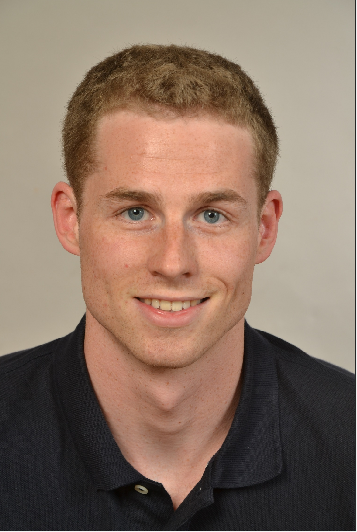
\includegraphics[height=4cm]{./img/ycbcr/tobi_WithoutThresholding}
}\subfigure[YCbCr color space]{
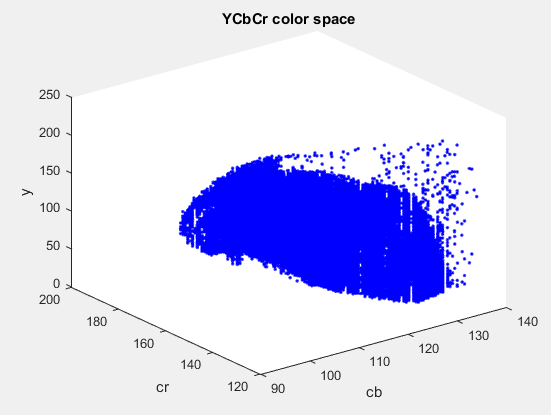
\includegraphics[height=4cm]{./img/ycbcr/Tobi_full}}
\caption{YCbCr - without Thresholding - MEM3 student}\label{YCbCr_tobi_withoutThresholding}
\end{figure}

By applying the determined thresholds(see section \ref{sec:ColorThre}) the skin pixels can be seen clustered in a region of the YCBCR space (see figure \ref{YCbCr_tobi_withThresholding}).

\begin{figure}[!h]
\centering
\subfigure[Thresholded picture]{
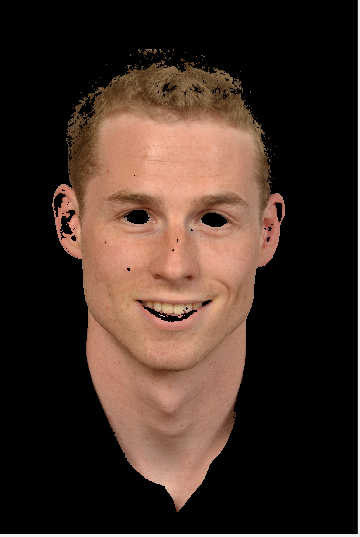
\includegraphics[height=4cm]{./img/ycbcr/tobi_Thresholding}
}\subfigure[YCbCr color space]{
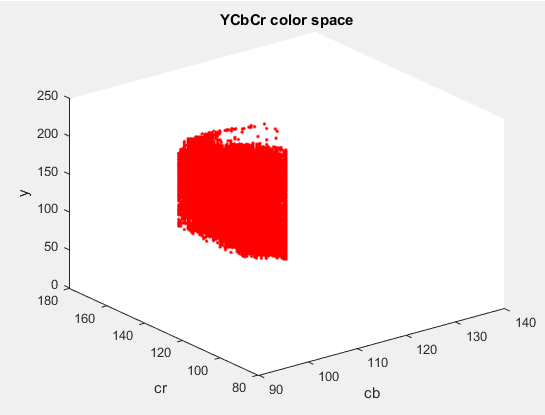
\includegraphics[height=4cm]{./img/ycbcr/Tobi_thresholding_3d_single}}
\caption{YCbCr - with Thresholding - MEM3 student}\label{YCbCr_tobi_withThresholding}
\end{figure}

\medskip
A comparison between the whole coloured picture and the threshold picture (see figure \ref{comparisonOfThresholding}) shows that the relevant information of the skin color is in the chrominance (Cb and Cr) and independent of the luminance (Y).

\begin{figure}[!h]
\centering
\subfigure[Thresholded picture]{
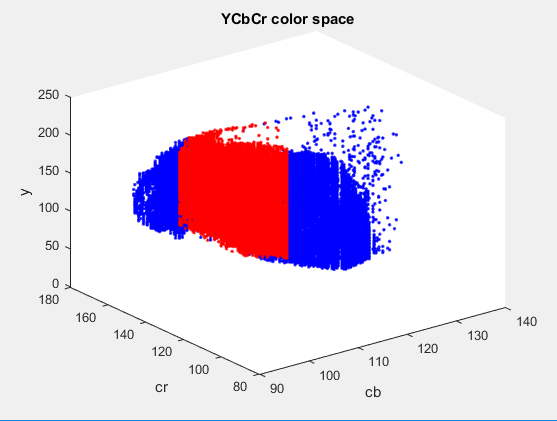
\includegraphics[height=4cm]{./img/ycbcr/Tobi_thresholding_3d}
}\subfigure[YCbCr color space]{
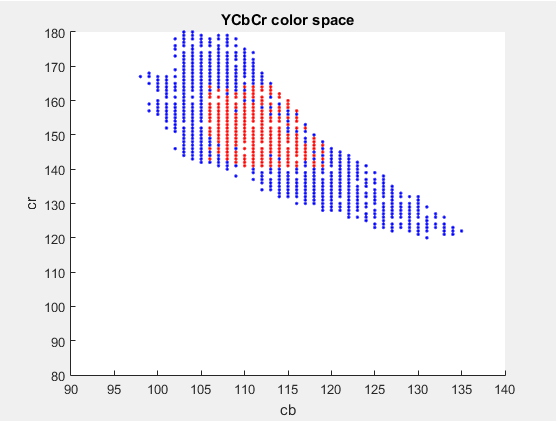
\includegraphics[height=4cm]{./img/ycbcr/Tobi_thresholding_cb_cr}}
\caption[YCbCr - comparison - full colored and thresholded]{YCbCr - comparison between the full colord picture (blue dots) and the thresholded picture (red dots) - MEM3 student}\label{comparisonOfThresholding}
\end{figure}

\medskip
Interesting is that independent of the skin type (white, black or yellow) the relevant skin pixels are always at the same region. To show this the pictures of figure \ref{testPictures} were thresholded and compared see figure yy.

\begin{figure}[!h]
\centering
\subfigure[MEM3 student]{
\includegraphics[height=3.5cm]{../../MATLAB/pictures/me1_mod}
}
\subfigure[Barack Obama]{
\includegraphics[height=3.5cm]{../../MATLAB/pictures/obama}}
\subfigure[Jackie Chan]{
\includegraphics[height=3.5cm]{../../MATLAB/pictures/JackieChan}}
\caption{Test pictures}\label{testPictures}
\end{figure}

\begin{figure}[!h]
\centering
\subfigure[Thresholded picture]{
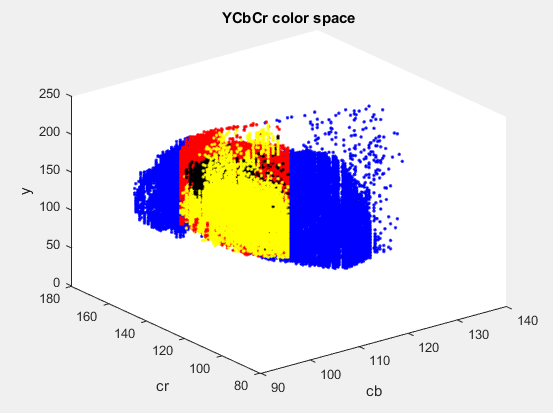
\includegraphics[height=4cm]{./img/ycbcr/Comparison_3Pics_3d}
}\subfigure[YCbCr color space]{
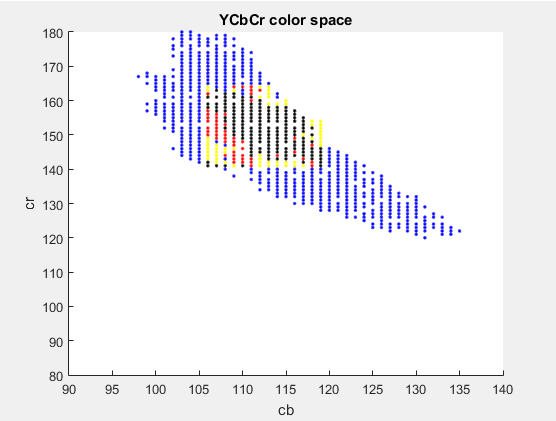
\includegraphics[height=4cm]{./img/ycbcr/Comparison_3Pics_cb_cr}}
\caption[YCbCr - comparison - MEM3 student, Chan and Obama]{YCbCr - comparison between the full colord picture of MEM3 student (blue dots), thresholded MEM3 student (red dots), thresholded Jackie Chan (yellow dots) and thresholded Barack Obama (black dots).}
\label{testPicturesComparison}
\end{figure}

\newpage

\section{Color threshold}\label{sec:ColorThre}  	
\subsection{Procedure}
According to different literature (Real Time Detection and Tracking of Human Face using Skin Color Segmentation and Region Properties \cite{RTFaceDetection}, Face Detection Using Color Thresholding, and Eigenimage Template Matching \cite{RTFaceDetection} and A Robust Skin Color Based Face Detection Algorithm \cite{RobustSkinColorFD}) the thresholds must be found with an try and error procedure.

The three mentioned articles have chosen different thresholds, in this project the thresholds were chosen with the MATLAB application colorThresholder (from the Image Processing Toolbox).

\medskip
To run this application the command \textit{colorThresholder} must be entered into the command window of MATLAB.

\medskip
After loading an image and choosing the color space (in this case the YCbCr space - see figure \ref{obamaOrig}) the thresholds can be set (see figure \ref{obamaThres}).

The next step is to use the find values for Cb and Cr:
\begin{itemize}
\item Cb: 105 $>$ Cb $<$ 120
\item Cr: 140 $>$ Cr $<$ 165
\end{itemize}

to threshold the image (values above the over limit and pixel values under the lower value will be set to black, all pixels within the limit will set to white). This can be done with the matlab commands:
\begin{lstlisting}
% Thresholding -> binary
thresh_cb = cb > 105 & cb < 120;    % thresholding for cb values
thresh_cr = cr > 140 & cr < 165;    % thresholding for cr values
binary_pic = thresh_cb&thresh_cr;   % create binary picture
\end{lstlisting}
The result looks like figure \ref{obamaBin}.

\medskip
The next steps is to modify the binary picture (by removing the small black pixels in the face and the small white pixels out of the face) to make face detection more efficient.

\begin{figure}[!h]
\centering
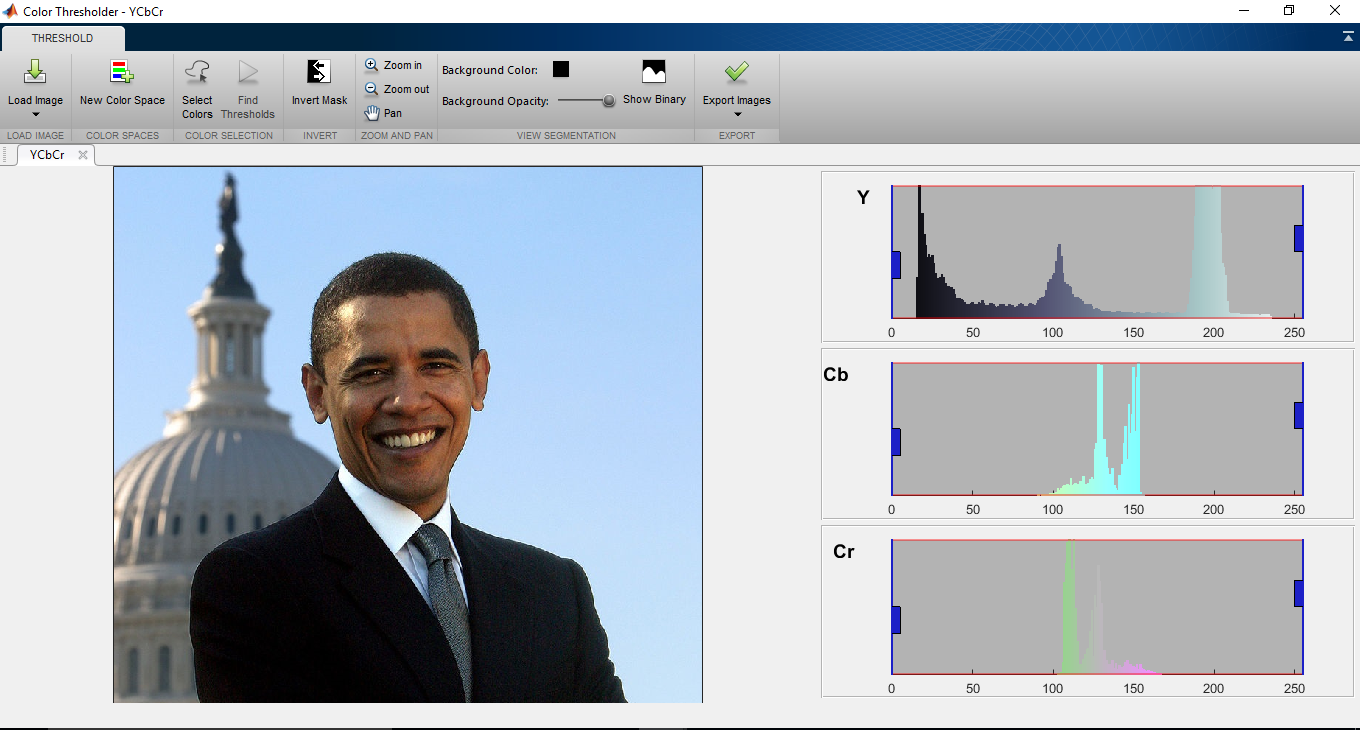
\includegraphics[width=5cm]{./img/thresholds/obama_orig.PNG}
\caption{colorThresholder - Barrack Obama - without thresholding}
\label{obamaOrig}
\end{figure}

\begin{figure}[!h]
\centering
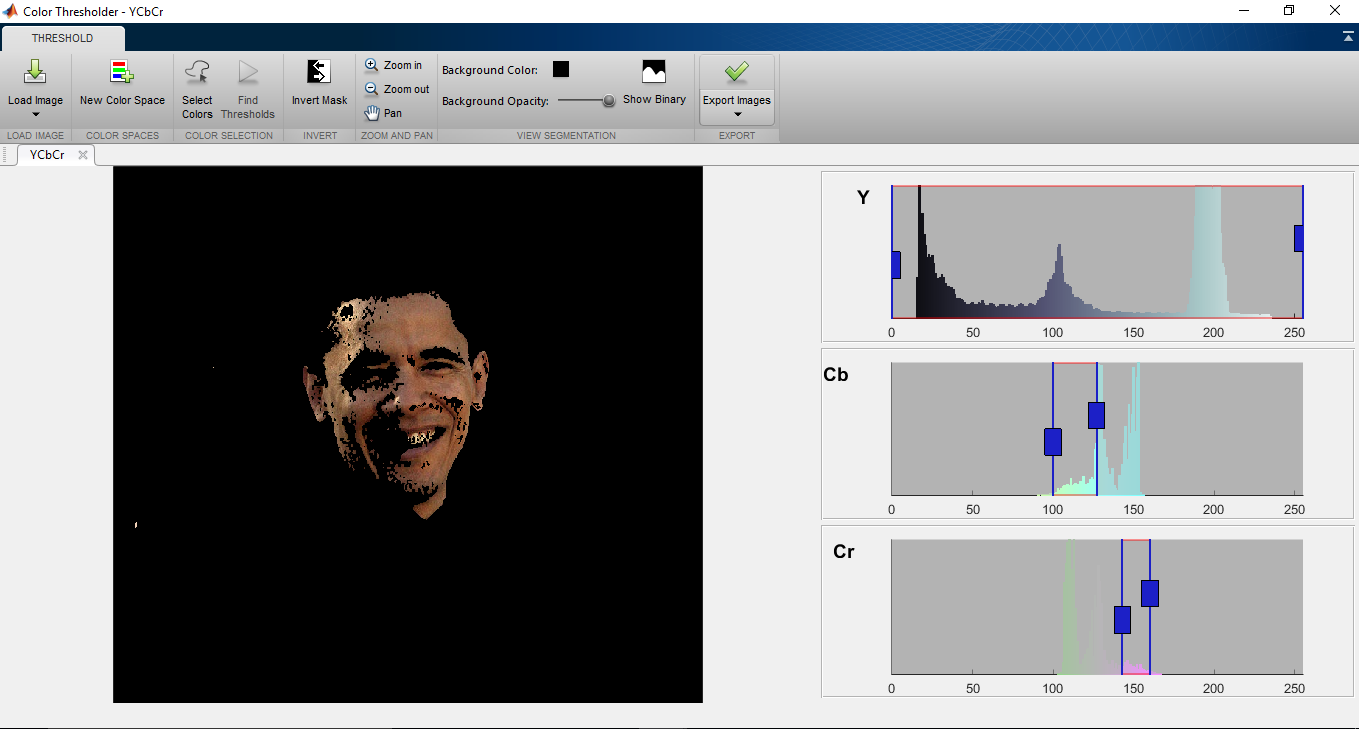
\includegraphics[width=10cm]{./img/thresholds/obama_thresholds.PNG}
\caption[colorThresholder - Barrack Obama - with thresholds]{colorThresholder - Barrack Obama - with thresholds : 105 $>$ cb $<$ 120 and 140 $>$ cr $<$ 165}
\label{obamaThres}
\end{figure}

\begin{figure}[!h]
\centering
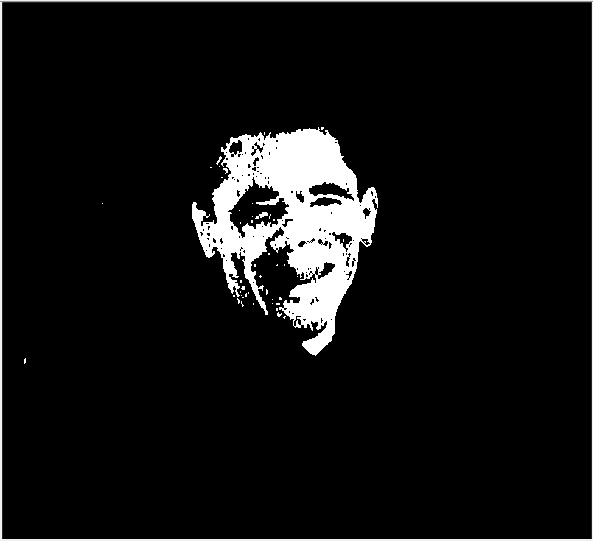
\includegraphics[width=8cm]{./img/thresholds/obama_thresholds_binary.PNG}
\caption{colorThresholder - Barrack Obama - with thresholds - Binary}
\label{obamaBin}
\end{figure}

\newpage
\subsection{MATLAB implementation}
\begin{lstlisting}[caption=Color thresholding, label= matlabColorTresholding]
I=imread('../pictures/obama.jpg');  % load image from workspace

% RGB -> YCbCr
YCBCR = rgb2ycbcr(I);               % transform image into YCbCr space
y = YCBCR(:,:,1);                   % extract Y value out of matrix
cb = YCBCR(:,:,2);                  % extract Cb value out of matrix
cr = YCBCR(:,:,3);                  % extract Cr value out of matrix

% Thresholding -> binary
thresh_cb = cb > 105 & cb < 120;    % thresholding for cb values
thresh_cr = cr > 140 & cr < 165;    % thresholding for cr values
binary_pic = thresh_cb&thresh_cr;   % create binary picture

% show binary picture:
figure
imshow(binary_pic);
\end{lstlisting}

\begin{figure}[!h]
\centering
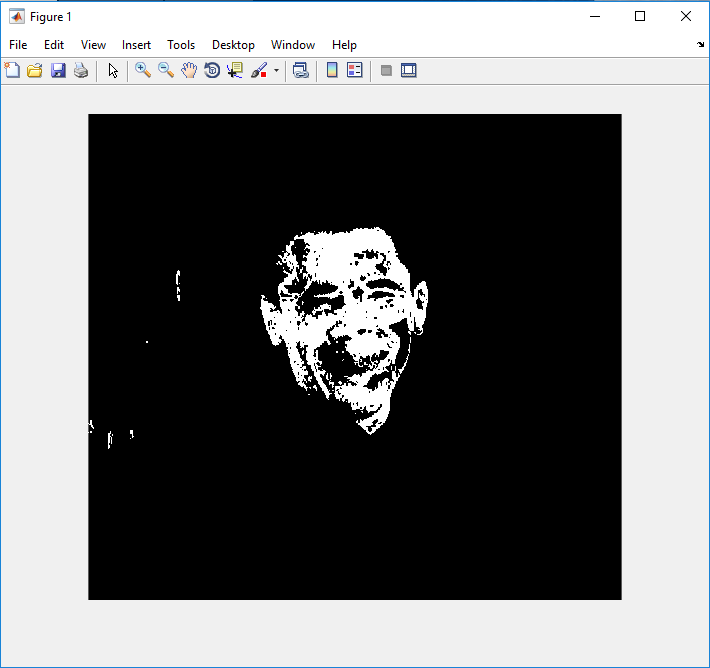
\includegraphics[width=10cm]{./img/thresholds/obama_matlab.PNG}
\caption[Binary Picture - Barrack Obama]{Binary Picture - Barrack Obama - figure out of matlab code \ref{matlabColorTresholding}}
\label{obamaThres}
\end{figure}

\subsection{Examples}

\begin{figure}[!h]
\centering
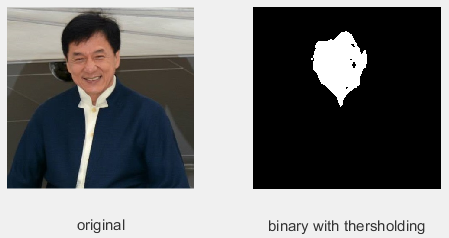
\includegraphics[height = 4cm]{./img/thresholds/chackie}
\caption{Chackie Jan}
\end{figure}

\begin{figure}[!h]
\centering
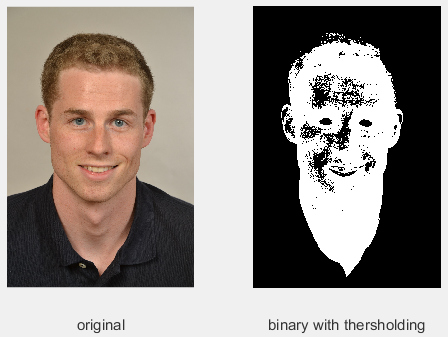
\includegraphics[height = 4cm]{./img/thresholds/tobiBu}
\caption{MEM student (private picture)}
\end{figure}
\begin{figure}[!h]
\centering
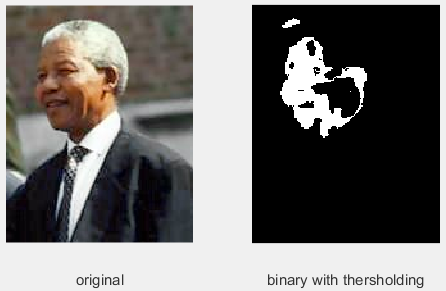
\includegraphics[height = 4cm]{./img/thresholds/mandela}
\caption{Nelson Mandela}
\end{figure}



	
\end{document}
